\chapter{Ejecución del proyecto}
\label{chap:edp}
Este capítulo tiene como objetivo tratar el desarrollo del proyecto en sí mismo, así como discutir las opciones disponibles durante el progreso y las decisiones tomadas para llevarlo a cabo.

\section{Consideraciones previas}
Este trabajo nace como un desarrollo del proyecto troncal de \citeauthor{IglesiasGuitian2022} y como tal se debe ceñir a las condiciones que acarrea dicho proyecto. Todo el equipo utilizado durante el desarrollo fue provisto por parte del mismo, o en su defecto por parte del \acrfull{citic}.

\section{Análisis}
Se llevó a cabo un estudio para definir la hoja de ruta del proyecto. Dada la problemática a solventar, este trabajo alcanza a tocar áreas bien diferenciadas entre si que se pueden destacar como los pasos a seguir del mismo:
\begin{itemize}
	\item Extracción de volúmenes 3D a partir de un \acrshort{tc} válidos para su impresión.
	\item Diseñar un marcador fiduciario que permita el seguimiento de una pieza en 3 dimensiones y un método de acople al volumen previamente impreso.
	\item Implementar una solución que permita el seguimiento de dicho marcador.
	\item Integrar la solución sobre un \acrshort{hmd}.
\end{itemize}

Fruto de la investigación surge el artículo de  \citeauthor{MoretaMartinez2020}; que expone una solución existente a los objetivos de este trabajo mediante el uso de software bajo licencia o de pago.  Es por ello que se toma una aproximación similar al problema, sobre todo en las fases iniciales, para la generación de los volúmenes a pesar de implementar una solución propia para lo que a seguimiento se refiere. Este estudio también permitió especificar los requisitos necesarios para el software de tracking.

Uno de los principales requisitos debe ser la robustez del sistema frente a las oclusiones del marcador. Es necesario que el seguimiento sea posible a pesar de la oclusión parcial del marcador. Además, es preciso que a partir de una fuente de vídeo se puedan extraer las coordenadas del marcador, así como su rotación en el espacio. Destacar también que el seguimiento debe ocurrir en un segundo plano, entorpeciendo lo menos posible las operaciones del hilo principal de ejecución, ya que parte de estas operaciones tiene una latencia crítica.

Este trabajo nace como un desarrollo del proyecto troncal de \citeauthor{IglesiasGuitian2022}, y como tal, debe ceñirse a ciertas pautas del mismo. Exposure Render cuenta con un módulo de realidad virtual, en el que se integrará la solución de tracking para lograr un control mas natural sobre el modelo a tratar, moviéndose en las imágenes renderizadas a la par que se mueve en la realidad, como se muestra en el diagrama de secuencia de la \figurename~\ref{fig:flow_exposure}.

\begin{figure}
	\centering
	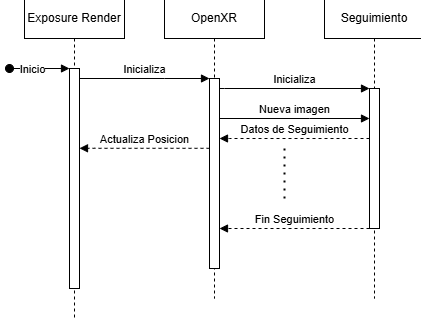
\includegraphics[width=0.75\textwidth]{imaxes/flow_exposure.png}
	\caption{Flujo de integración del seguimiento en Exposure Render.}
	\label{fig:flow_exposure}
\end{figure}

\section{Generación de volúmenes a partir de TC}
Con el fin de facilitar la validación del progreso del proyecto, se utilizó una \acrshort{tc} de pruebas. Dichos datos contienen la sección superior (hombros y cabeza) de un sujeto, mostrado en la \figurename~\ref{fig:manix_full}. Durante el desarrollo se sugirió como posible caso práctico seleccionar el cráneo del sujeto en los datos de prueba y trabajar en la alineación 3D sobre el mismo.
%En las siguientes figuras se representa este objetivo.

% \begin{figure}
%   \centering
%   \includegraphics[width=0.4\textwidth]{imaxes/manix_full.png}
%   \caption{Datos de prueba.}
%   \label{fig:manix_full}
% \end{figure}

Con el fin de seleccionar una sección concreta para exportar, se utilizaron las herramientas para segmentar volúmenes de Slicer3D.
Al abrir el programa se pueden ver las vistas, en las que se representará el \acrshort{tc} una vez cargado, como se muestra en la captura de pantalla de la \figurename~\ref{fig:3dslier}.
Se utilizo principalmente la herramienta de ``Thresholding'' que permite seleccionar partes del modelo cuyas intensidades se comprenden en un intervalo o ``threshold'' (ver \figurename~\ref{fig:seg_cr}). Posteriormente, para la eliminación de las partes del modelo no deseadas, se utilizó la herramienta de borrado hasta alcanzar el volumen deseado.

\begin{figure}
	\centering
	\begin{subfigure}{.4\textwidth}
		\includegraphics[width=\textwidth]{imaxes/manix_full.png}
		\caption{TC usado en el desarrollo.}\label{fig:manix_full}
	\end{subfigure}
	\begin{minipage}[b]{.47\textwidth}
		\begin{subfigure}{\textwidth}
			\centering
			\includegraphics[width=\textwidth]{imaxes/captura3dslicer_2.png}
			\caption{ Captura de pantalla de 3DSlicer con los datos cargados.}\label{fig:3dslier}
		\end{subfigure}\\
		\begin{subfigure}{\textwidth}
			\centering
			\includegraphics[width=\textwidth]{imaxes/segment_craneo.png}
			\caption{ Captura de pantalla de 3DSlicer del torso una vez aplicado el thresholding.}\label{fig:seg_cr}
		\end{subfigure}
	\end{minipage}
	\caption{\acrshort{tc} de partida y obtención del modelo 3D final con 3DSlicer.}
\end{figure}

\section{Impresión 3D del volumen}
Durante el proceso de segmentación y exportación del modelo, pueden surgir inconsistencias geométricas debido a que el modelo se genera directamente de los datos volumétricos del TC, en lugar de construirse a partir de primitivas geométricas predefinidas. Estas irregularidades, que incluyen superficies no continuas o vértices mal conectados, impedirían un correcto proceso de Slicing y, por consiguiente, la generación adecuada del archivo GCODE necesario para la impresión 3D. Para solucionar este problema, se utilizó el software Meshmixer, una herramienta especializada en la reparación y optimización de mallas 3D. Como se muestra en la \figurename~\ref{fig:arr_geo}, el modelo exportado presenta varios puntos problemáticos, señalados por marcadores, que corresponden a errores geométricos derivados del proceso de exportación. Una vez corregidos estos defectos mediante las herramientas de reparación de Meshmixer, el modelo quedó preparado para su impresión.

\begin{figure}
	\centering
	\includegraphics[width=0.6\textwidth]{imaxes/arreglo_geo.png}
	\caption{Modelo de cráneo 3D con geometrías erróneas.}
	\label{fig:arr_geo}
\end{figure}

Como se comenta en el Capítulo \ref{chap:hs}, para una pieza con una geometría tan compleja, se requeriría una gran cantidad de soportes. Debido a esto, se optó por la impresora Fuse 1 para la impresión de este modelo. A diferencia de una impresora 3D al uso, esta impresora utiliza un láser para fijar capa a capa el polvo de nylon, lo que garantiza una gran resolución en la pieza final y una gran durabilidad de la misma.

Posterior al  trabajo de impresión es necesario retirar el material sobrante en la cámara de recuperación que cuenta con distintos utensilios para evitar malgastar el material sobrante ya que puede ser reutilizado.

\begin{figure}%
	\centering
	\subfloat[\centering Pieza en el proceso de recuperación del material.]{{\includegraphics[width=.4\textwidth]{imaxes/limpiando_fig.png} }}%
	\qquad
	\subfloat[\centering  Pieza final.]{{\includegraphics[width=.4\textwidth]{imaxes/limpia_fig.png} }}%
	\caption{Proceso de recuperación de material.}%
	\label{fig:limpieza}%
\end{figure}

\section{Desarrollo del marcador fiduciario}
\label{sec:marcador_fiduciario}

\subsection{Planteamiento del problema y selección de la solución}
Obtener la posición y rotación de una figura desconocida en el espacio es uno de los problemas principales a la hora de implementar soluciones de realidad virtual o aumentada, ya que requiere encontrar correspondencias entre objetos conocidos en el espacio y sus proyecciones en el vídeo.

Si bien existen aproximaciones que buscan puntos claves de las figuras o reconocen sus geometrías mediante técnicas de visión artificial e inteligencia artificial, se optó por el uso de  marcadores fiduciarios por varios motivos:

\begin{itemize}
    \item \textbf{Independencia del hardware}: Permite replicar el seguimiento del objeto independientemente del hardware utilizado, ya que una vez calibrada la cámara no se requiere ningún otro tipo de ajuste en el sistema.
    \item \textbf{Robustez frente a oclusiones}: Permite mantener el seguimiento a pesar de que parte del marcador se encuentre ocluido o no esté completamente en el campo de visión de la cámara.
    \item \textbf{Simplicidad de implementación}: Dados los recursos disponibles, se optó por utilizar la librería ARuco para generar y seguir el marcador, aprovechando su madurez y estabilidad.
\end{itemize}

\subsection{Fundamentos teóricos del seguimiento con ARuco}

ARuco a la hora de detectar la posición de un marcador, trabaja con un modelo de coordenadas pin-hole, donde las coordenadas y rotación de los objetos detectados se expresan en función de la posición de la cámara.
El calibrado de la cámara permite determinar la proyección de cualquier punto en las 3 dimensiones del espacio en el sensor de la cámara. En una cámara ideal, un punto 3D $(X, Y, Z)$ en el espacio se proyectaría en el píxel:
\begin{align*}
	x & = \frac{X \cdot fx}{Z} + cx & y = \frac{Y \cdot fy}{Z} + cy
\end{align*}
Donde:
\begin{itemize}
	\item $fx$, $fy$: Es la longitud focal de la lente de la cámara en ambos ejes.
	\item $cx$, $cy$: Es el centro óptico del sensor (expresado en píxeles).
	\item $k1$, $k2$, $p1$, $p2$, $k3$: Son los coeficientes de distorsión radial y tangencial que permiten corregir las distorsiones introducidas por la lente real.
\end{itemize}
Asumiendo que la ubicación tridimensional del punto con respecto al sistema de referencia de la cámara es conocida. Si se desea conocer la proyección de un punto referido a un sistema de referencia arbitrario, entonces deben mencionarse parámetros extrínsecos. Los parámetros extrínsecos consisten básicamente en las rotaciones tridimensionales (Rvec = {Rx, Ry, Rz}) y las traslaciones tridimensionales (Tvec = {Tx, Ty, Tz}) requeridas para trasladar el sistema de referencia de la cámara al sistema arbitrario. Los elementos de rotación se expresan mediante la fórmula de Rodrigues \cite{mebius2007derivation}, por lo que es posible obtener la matriz de rotación equivalente de 3x3 utilizando la función cv::Rodrigues() de OpenCV.

Cada marcador detectado devuelve como coordenadas la esquina superior izquierda del mismo, o lo que se etiqueta en el ejemplo de la \figurename~\ref{fig:marker_schema} como \emph{corner 0}, en forma de (Rvec = {Rx, Ry, Rz}) como vector de rotación y (Tvec = {Tx, Ty, Tz}) como vector de translación.

\begin{figure}
	\centering
	\includegraphics[width=0.5\textwidth]{imaxes/marker_schema.png}
	\caption{Esquema de un marcador.}
	\label{fig:marker_schema}
\end{figure}

Detectar un solo marcador puede fallar por diferentes razones, como malas condiciones de iluminación, movimiento rápido de la cámara, obstrucciones, etc. Para superar ese problema, ArUco permite el uso de tablas de marcadores como la mostrada en la \figurename~\ref{fig:board_schema}. Cada tabla de marcadores está compuesta por varios marcadores en ubicaciones conocidas. Presentan dos ventajas principales. Primero, dado que hay más de un marcador, es menos probable perderlos todos de vista al mismo tiempo. Segundo, cuanto más marcadores se detecten, más puntos están disponibles para calcular los parámetros extrínsecos de la cámara. Como consecuencia, se obtiene una mayor precisión.

\begin{figure}
	\centering
	\includegraphics[width=0.4\textwidth, angle=90]{imaxes/board_schema.png}
	\caption{Esquema de una tabla de marcadores.}
	\label{fig:board_schema}
\end{figure}

\subsection{Generación de marcadores a partir de diccionarios predefinidos}
El marcador fiduciario utilizado en este proyecto se genera a partir de un diccionario predefinido de ArUco. En la implementación actual se emplea el diccionario \texttt{DICT\_6X6\_250}, que contiene 250 marcadores únicos de 6×6 bits cada uno. Este diccionario fue seleccionado por ofrecer un buen equilibrio entre:

\begin{itemize}
    \item \textbf{Robustez en la detección}: Los marcadores de 6×6 bits proporcionan suficiente información para una detección fiable incluso con cierta degradación de la imagen.
    \item \textbf{Capacidad del diccionario}: Con 250 marcadores únicos disponibles, hay suficientes IDs para implementar múltiples cubos sin conflictos.
    \item \textbf{Replicabilidad}: Al usar un diccionario estándar, los experimentos son fácilmente reproducibles.
\end{itemize}

La generación del cubo marcador sigue un esquema sistemático donde cada cara del cubo contiene una matriz 2×2 de marcadores del mismo diccionario. Los identificadores (IDs) de los marcadores se asignan secuencialmente siguiendo la fórmula:

\begin{center}
\texttt{firstId = cara\_id * 4}\\
\texttt{ids = \{firstId, firstId + 1, firstId + 2, firstId + 3\}}
\end{center}

Donde \texttt{cara\_id} corresponde al número de cara del cubo (0-5). De esta forma:
\begin{itemize}
	\item Cara 0: marcadores con IDs 0, 1, 2, 3
	\item Cara 1: marcadores con IDs 4, 5, 6, 7
	\item Cara 2: marcadores con IDs 8, 9, 10, 11
	\item Cara 3: marcadores con IDs 12, 13, 14, 15
	\item Cara 4: marcadores con IDs 16, 17, 18, 19
	\item Cara 5: marcadores con IDs 20, 21, 22, 23
\end{itemize}

Esta implementación permite utilizar cualquier diccionario predefinido o personalizado de ArUco, siempre y cuando el diccionario contenga al menos 24 marcadores únicos y se respete el orden secuencial de asignación de IDs para cada cara. La modularidad del sistema permite cambiar el diccionario sin necesidad de alterar la lógica de seguimiento del cubo.

\subsection{Algoritmo de cálculo de pose del cubo}
\label{subsec:algoritmo_pose}

El proceso de determinación de la pose del cubo se realiza en varias etapas que transforman las detecciones individuales de cada cara en una pose unificada del centro del cubo.

\subsubsection{Transformación de coordenadas de cara a centro}
Cuando ARuco detecta una cara del cubo, devuelve la posición y orientación correspondientes a la esquina superior izquierda de esa cara (corner 0 en la \figurename~\ref{fig:marker_schema}). Para obtener la pose del centro del cubo, es necesario aplicar una transformación que tenga en cuenta tanto la posición como la orientación actual del marcador.

\subsection{Diseño geométrico del marcador cúbico}

Debido a la versatilidad de las piezas con las que se pretende usar el marcador, se implementó priorizando eliminar las oclusiones del marcador por la pieza. Por este motivo se diseñó como un cubo, de forma que al menos una cara sería visible en todo momento. Se evaluaron otras formas geométricas (prismas rectangulares, pirámides, cilindros), pero estas demostraron menor efectividad de detección con la cámara utilizada en el desarrollo.

El diseño final consiste en un cubo donde cada cara contiene una matriz 2×2 de marcadores del mismo diccionario ARuco. Esta configuración proporciona las siguientes ventajas:

\begin{itemize}
    \item \textbf{Redundancia}: Al tener múltiples marcadores por cara, el sistema puede mantener el tracking incluso si algunos marcadores están ocluidos.
    \item \textbf{Precisión mejorada}: La detección de múltiples marcadores en la misma cara permite calcular la pose con mayor precisión mediante promediado.
    \item \textbf{Robustez}: La forma cúbica garantiza que siempre habrá al menos una cara visible desde cualquier ángulo de observación.
\end{itemize}

Se llevaron a cabo pruebas con distintos diccionarios de marcadores, modificando las tolerancias para los márgenes entre marcadores y los bordes del cubo con el fin de poder mantener unas dimensiones manejables sin comprometer el tamaño de cada marcador individual.
Finalmente, fruto de los tests, se llegó al cubo de la \figurename~\ref{fig:cubo_marker}.

El cubo se descompone como se puede ver en la \figurename~\ref{fig:cube_layout}. En un primer momento la detección devuelve la posición y rotación de cada cara de forma individual. Dado que se busca la posición del centro del cubo, sobre cada valor obtenido, se aplica una transformación que tiene en cuenta tanto la posición como la orientación actual del marcador. La función \texttt{moveAxis} calcula el desplazamiento necesario para cada eje utilizando la matriz de rotación (obtenida mediante la fórmula de Rodrigues) para asegurar que el desplazamiento se realiza en la dirección correcta respecto a la orientación actual del marcador. Este proceso se aplica para los tres ejes como se muestra a continuación:

\begin{figure}
	\centering
	\includegraphics[width=0.4\textwidth]{imaxes/cube_layout.png}
	\caption{Layout de las caras del marcador fiduciario.}
	\label{fig:cube_layout}
\end{figure}

\begin{lstlisting}[language=C++]
cv::Vec3d moveAxis(cv::Vec3d& tvec, cv::Vec3d rvec, double distance, int axis)
{
    cv::Mat rotationMatrix, rotationMatrixTransposed;
    Rodrigues(rvec, rotationMatrix);
    rotationMatrixTransposed = rotationMatrix.t();
    double* rz = rotationMatrixTransposed.ptr<double>(axis); // x=0, y=1, z=2
    tvec[0] -= rz[0] * distance;
    tvec[1] -= rz[1] * distance;
    tvec[2] -= rz[2] * distance;
    return tvec;
}
tvecs = moveAxis(tvecs, rvecs, -SIDELENGTH, 0);
tvecs = moveAxis(tvecs, rvecs, -SIDELENGTH, 1);
tvecs = moveAxis(tvecs, rvecs, -SIDELENGTH, 2);

\end{lstlisting}

Una vez ajustada la posición del centro, es necesario corregir la orientación de cada cara para mantener un sistema de coordenadas consistente en todo el cubo. La función \texttt{cubeCoordinates} aplica las rotaciones necesarias según la cara detectada, usando la cara 0 como referencia. Las rotaciones se realizan sobre los ejes X, Y, y Z mediante las funciones \texttt{rotateXAxis}, \texttt{rotateYAxis}, y \texttt{rotateZAxis}, que aplican transformaciones angulares usando radianes (donde $\pi$ radianes equivale a 180 grados):
\begin{lstlisting}[language=C++]
void cubeCoordinates(int id, cv::Vec3d& rvecs, cv::Vec3d& tvecs, float sideLength)
{
    tvecs = moveAxis(tvecs, rvecs, -SIDELENGTH, 0);
    tvecs = moveAxis(tvecs, rvecs, -SIDELENGTH, 1);
    tvecs = moveAxis(tvecs, rvecs, -SIDELENGTH, 2);
    switch (id)
    {
    case 1://cara 1
        rvecs = rotateXAxis(rvecs, -M_PI / 2);
        break;
    case 2://cara 2
        rvecs = rotateXAxis(rvecs, M_PI);
        break;
    case 3://cara 3
        rvecs = rotateYAxis(rvecs, M_PI / 2);
        rvecs = rotateZAxis(rvecs, M_PI);
        break;
    case 4://cara 4
        rvecs = rotateXAxis(rvecs, M_PI);
        rvecs = rotateYAxis(rvecs, -M_PI / 2);
        break;
    case 5://cara 5
        rvecs = rotateXAxis(rvecs, M_PI / 2);
        break;
    default://La cara 0 no precisa rotar
        break;
    }
}
\end{lstlisting}

\subsubsection{Fusión de múltiples detecciones}
Cuando se detectan múltiples caras del cubo simultáneamente (hasta 3 caras pueden ser visibles en una sola imagen), el sistema debe combinar las estimaciones individuales para obtener una pose más precisa y estable. El algoritmo implementado utiliza un promediado simple de los vectores de traslación y rotación.

El promediado de vectores de rotación requiere especial atención debido a la naturaleza circular de las rotaciones y posibles discontinuidades en la representación de Rodrigues. El sistema implementa verificaciones para evitar promediar rotaciones que difieran significativamente, lo que podría indicar detecciones erróneas o ambigüedades en la orientación.


\begin{figure}%
	\centering
	\subfloat[\centering Modelo del marcador fiduciario.]{{\includegraphics[width=6cm]{imaxes/cubo_marker.png} }}%
	\qquad
	\subfloat[\centering  Impresión del marcador fiduciario.]{{\includegraphics[width=6cm]{imaxes/cubo_marker_imp.png} }}%
	\caption{Diseño final del marcador fiduciario.}%
	\label{fig:cubo_marker}%
\end{figure}

En caso de que únicamente se detectase una cara del cubo, los vectores de rotación y translación finales serían los obtenidos llegados a este punto. Como se observa en la \figurename~\ref{fig:cubo_detected}, es posible detectar hasta 3 caras simultáneamente en una única imagen, lo que permite aplicar el algoritmo de fusión descrito anteriormente para obtener una estimación más robusta de la pose.

\begin{figure}%
	\centering
	\subfloat[\centering Ejemplo de detección del cubo.]{{\includegraphics[width=6cm]{imaxes/cube_detected.png} }}%
	\qquad
	\subfloat[\centering Ejemplo de detección del cubo con oclusión.]{{\includegraphics[width=6cm]{imaxes/cube_detected_ocluded.png} }}%
	\caption{Imágenes sobre las que se estima la pose del cubo.}%
	\label{fig:cubo_detected}%
\end{figure}

\subsubsection{Procesamiento de secuencias de vídeo}
Hasta ahora, se ha descrito el comportamiento de la aplicación para una única imagen. El procesamiento de secuencias de vídeo consiste en aplicar iterativamente este algoritmo a cada frame de la secuencia. Una vez obtenidos los valores de pose para un frame, el sistema espera al siguiente frame y ejecuta nuevamente el pipeline de detección. En la \figurename~\ref{fig:flujo_tfg} se ilustra el flujo completo del algoritmo, desde la captura de imagen hasta la obtención de la pose final del cubo.

El diagrama muestra claramente las etapas principales del proceso implementado:
\begin{enumerate}
    \item \textbf{Inicialización del sistema}: Apertura de la cámara, carga de parámetros de calibración, creación de las tablas de marcadores para cada cara del cubo e inicialización del detector ARuco.
    \item \textbf{Captura de frame}: Obtención del frame de vídeo desde la cámara.
    \item \textbf{Detección de marcadores}: Identificación inicial de marcadores ARuco en la imagen.
    \item \textbf{Refinamiento de detección}: Mejora de la precisión de detección aplicando el refinamiento específico para cada tabla de marcadores del cubo.
    \item \textbf{Procesamiento por cara}: Para cada una de las seis caras del cubo, se calculan las correspondencias entre puntos de imagen y puntos del objeto 3D.
    \item \textbf{Cálculo de pose individual}: Estimación de pose mediante solvePnP para cada cara que tenga correspondencias válidas.
    \item \textbf{Transformación al centro}: Conversión de las coordenadas de cada cara al centro del cubo utilizando las transformaciones geométricas correspondientes.
    \item \textbf{Promediado de poses}: Combinación de todas las poses válidas obtenidas para generar una estimación final más robusta.
    \item \textbf{Comunicación de resultados}: Retorno de la pose final calculada o pose vacía si no se detectaron marcadores.
\end{enumerate}

\begin{figure}
	\centering
	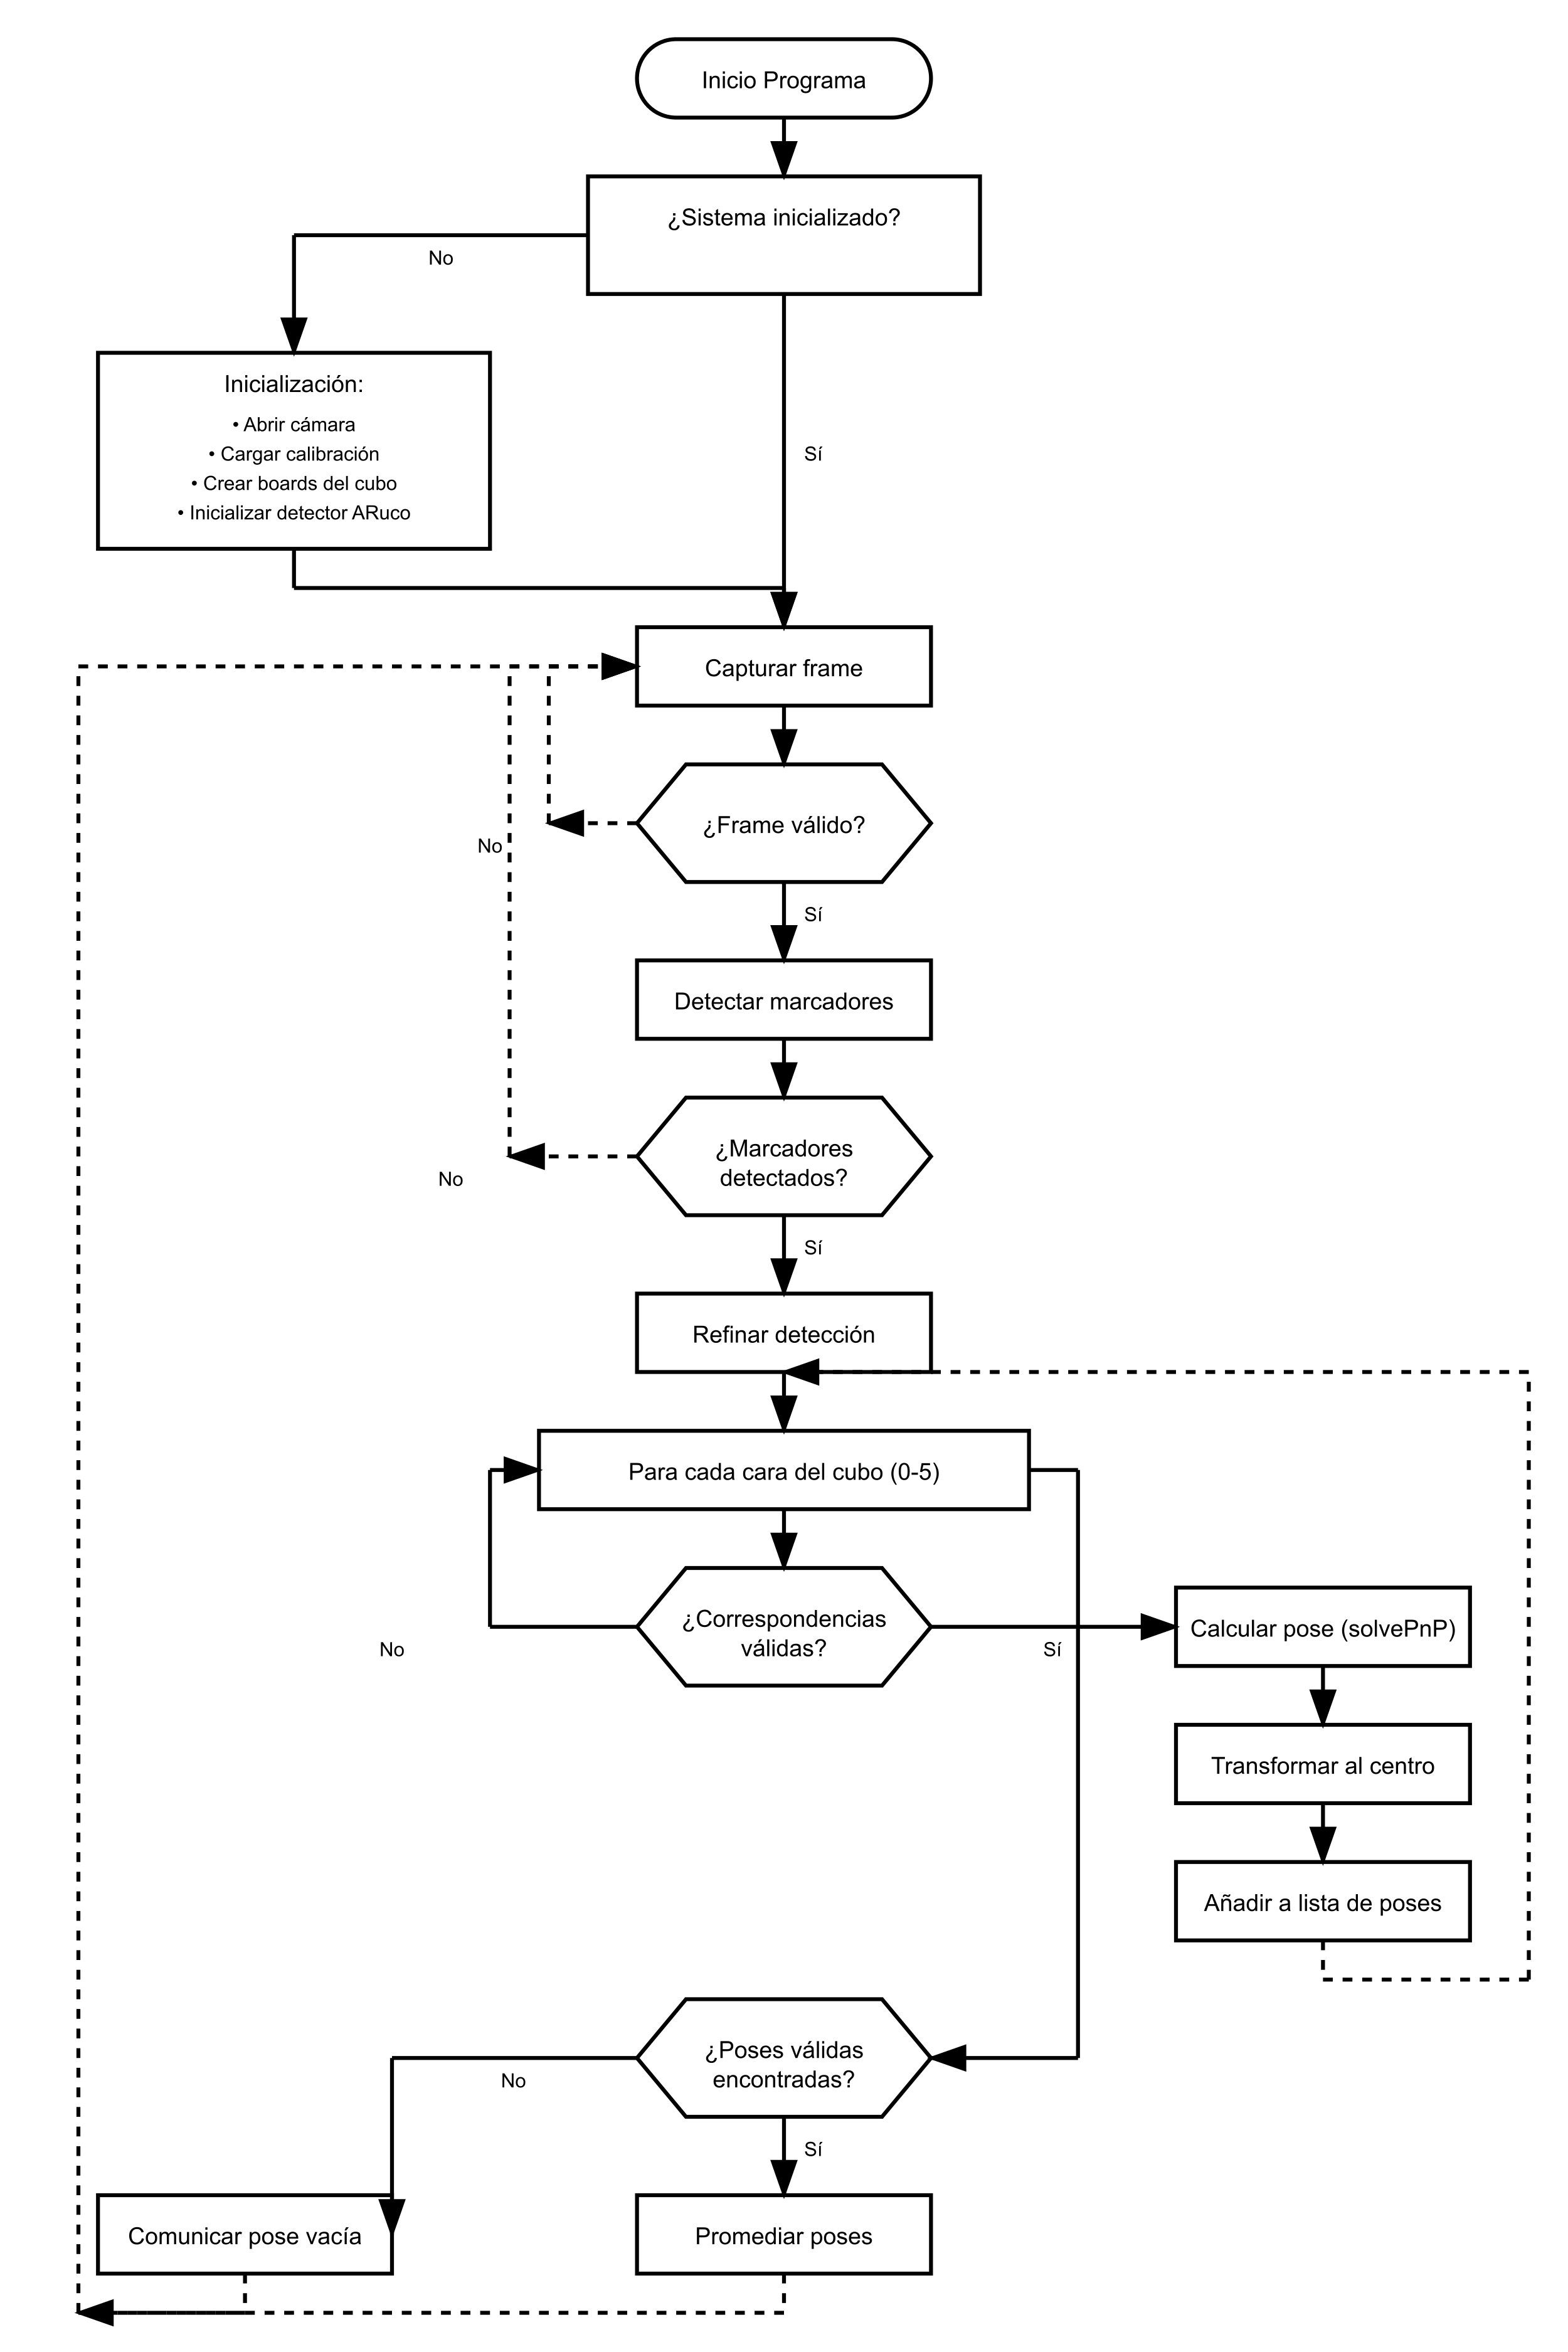
\includegraphics[width=0.8\textwidth]{imaxes/flujo_tfg_correcto.png}
	\caption{Diagrama de flujo de la solución de tracking implementada.}
	\label{fig:flujo_tfg}
\end{figure}

\section{Implementación del Passthrough en Exposure Render}
\subsection{Captura de imagen}
En un primer momento para la obtención de imágenes sobre las que poder realizar el seguimiento del marcador fiduciario se pretendían usar las propias cámaras frontales del HTC Vive Pro 2. Se trata de un par de cámaras colocadas longitudinalmente a lo largo del frontal del casco, que permiten su uso en aplicaciones de realidad aumentada y realidad mixta.
Se trato de acceder a las mismas mediante el uso de SRworks C++ SDK y con librerías de terceros a pesar de no tener éxito. Posteriormente tras conversaciones con el equipo de sorporte se concluyó que no era posible el acceso a las cámaras de forma nativa. Solo a través de Android o Unity en su defecto, lo que nos hizo descartar esta posibilidad.
La alternativa era acceder a las imágenes a través de una cámara de terceros. Esta opción presentaba la desventaja de imposibilitar el tratamiento de la imagen directamente en GPU, pero era la única viable.

\subsection{Integración del seguimiento}
Con el fin de no aumentar la cantidad de dependencias de un proyecto de la envergadura de Exposure Render, se trató de implementar la solución de tracking como una librería independiente que se pudiera integrar en el proyecto.

La integración del sistema de tracking ARuco en Exposure Render se realizó como una librería independiente que proporciona la funcionalidad de seguimiento de marcadores fiduciarios. El punto central de esta integración es la función \texttt{getCubePoseMatrix}, que actúa como interfaz principal entre el sistema de tracking y la aplicación de realidad aumentada.

\subsubsection{Función getCubePoseMatrix}
La función \texttt{getCubePoseMatrix} es la interfaz principal que proporciona la pose del cubo marcador en el espacio tridimensional:

\begin{lstlisting}[language=C++]
PoseMatrix4x4 getCubePoseMatrix(
    bool showVisualization,
    double markerSideLength,
    double markerGapLength,
    const std::string& calibrationFilePath,
    const std::string& boardDirPath,
    ImageData& undistortedImage);
\end{lstlisting}

Los parámetros de esta función tienen los siguientes propósitos:

\begin{itemize}
    \item \textbf{showVisualization}: Activa o desactiva la visualización en tiempo real del tracking para fines de depuración y validación.
    \item \textbf{markerSideLength}: Especifica la longitud física del lado de cada marcador individual en metros, necesaria para calcular la escala correcta.
    \item \textbf{markerGapLength}: Define la separación física entre marcadores en la superficie del cubo, utilizada para determinar las dimensiones reales del objeto.
    \item \textbf{calibrationFilePath}: Ruta al archivo de calibración de la cámara que contiene los parámetros intrínsecos y de distorsión.
    \item \textbf{boardDirPath}: Directorio que contiene las definiciones de las tablas de marcadores para cada cara del cubo.
    \item \textbf{undistortedImage}: Referencia de salida que contiene la imagen procesada y corregida para su uso en visualización.
\end{itemize}

\subsubsection{Implementación como hilo independiente}
Para minimizar la latencia y mantener la fluidez del renderizado principal, el sistema de tracking se implementó como un hilo independiente mediante la clase \texttt{Tracking} que encapsula toda la funcionalidad de seguimiento.

El flujo de ejecución del tracking opera en un hilo separado (\texttt{poseThread}) que ejecuta continuamente el siguiente proceso:

\begin{enumerate}
    \item \textbf{Captura de pose del headset}: Obtiene la matriz de transformación actual del casco VR desde el sistema OpenXR.
    \item \textbf{Captura de imagen}: Adquiere una nueva imagen desde la cámara del sistema.
    \item \textbf{Procesamiento de marcadores}: Ejecuta la detección y seguimiento de marcadores ARuco llamando a \texttt{getCubePoseMatrix}.
    \item \textbf{Sincronización de datos}: Actualiza de forma thread-safe la pose más reciente del cubo y la imagen procesada.
    \item \textbf{Actualización del overlay}: Envía la imagen procesada al sistema de overlay para visualización en realidad aumentada.
\end{enumerate}

La gestión de concurrencia utiliza mecanismos de sincronización para garantizar la integridad de los datos compartidos:
\begin{itemize}
    \item \textbf{std::mutex}: Protege el acceso a las variables \texttt{\_latestPose} y \texttt{\_latestCameraImage}.
    \item \textbf{std::atomic<bool>}: Controla el estado de ejecución del hilo mediante \texttt{\_poseThreadRunning}.
    \item \textbf{Lock guards}: Garantizan el acceso exclusivo durante las operaciones de lectura y escritura de datos compartidos.
\end{itemize}

Esta arquitectura asegura que el hilo principal de renderizado no se vea bloqueado por las operaciones de procesamiento de imagen, manteniendo una alta tasa de refresco en la experiencia de realidad aumentada mientras proporciona datos de tracking actualizados de forma continua.

\subsubsection{Estructura de datos PoseMatrix4x4 y transformaciones de coordenadas}

Para facilitar la integración con Exposure Render, la librería de tracking utiliza la estructura \texttt{PoseMatrix4x4}, que representa una matriz de 4×4. Esta estructura encapsula tanto la rotación como la traslación del marcador en el espacio 3D.

La función \texttt{getCubePoseMatrix} implementa una serie de transformaciones para que la pose del cubo detectada por ARuco sea directamente utilizable por el motor de renderizado de Exposure Render. El proceso de transformación se desarrolla en las siguientes etapas:

\paragraph{Transformación del espacio de cámara al espacio del cubo}
ARuco proporciona la pose del marcador como vectores de rotación y traslación (\texttt{rvec}, \texttt{tvec}) que representan la transformación del sistema de coordenadas del objeto al sistema de coordenadas de la cámara. Estos vectores se convierten en una matriz de transformación 4×4 usando la fórmula de Rodrigues para la rotación:

\begin{lstlisting}[language=C++]
cv::Mat cubeTransform = buildTransformation(rvecFinal, tvecFinal);
\end{lstlisting}

Esta matriz representa la transformación \gls{viewmatrix} del cubo respecto a la cámara.

\paragraph{Inversión para obtener la matriz modelo}
Para obtener la pose del cubo en el espacio de coordenadas de la cámara, es necesario invertir la matriz de transformación obtenida de ARuco. Esta inversión convierte la \gls{viewmatrix} en una \gls{modelmatrix} que describe la posición y orientación del cubo:

\begin{lstlisting}[language=C++]
cv::Mat cubeModel;
cv::invert(cubeTransform, cubeModel);
\end{lstlisting}

\paragraph{Conversión de sistemas de coordenadas}
OpenCV utiliza un sistema de coordenadas con matrices almacenadas en orden \gls{rowmajor}, mientras que \acrshort{osg} (utilizado por Exposure Render) emplea el orden \gls{columnmajor}. Para compatibilizar ambos sistemas, se aplica una transposición a la matriz.
\begin{lstlisting}[language=C++]
cv::Mat cubeModelTransposed;
cv::transpose(cubeModel, cubeModelTransposed);
\end{lstlisting}
Para ilustrar esta diferencia, consideremos una matriz de rotación 3×3:
$$
\begin{pmatrix}
r_{00} & r_{01} & r_{02} \\
r_{10} & r_{11} & r_{12} \\
r_{20} & r_{21} & r_{22}
\end{pmatrix}
$$

En el sistema \textbf{\gls{rowmajor}} (OpenCV), los elementos se almacenan en memoria fila por fila:
$$\text{Posición en memoria: } [r_{00}, r_{01}, r_{02}, r_{10}, r_{11}, r_{12}, r_{20}, r_{21}, r_{22}]$$

En el sistema \textbf{\gls{columnmajor}} (\acrshort{osg}), los elementos se almacenan columna por columna:
$$\text{Posición en memoria: } [r_{00}, r_{10}, r_{20}, r_{01}, r_{11}, r_{21}, r_{02}, r_{12}, r_{22}]$$

Esta diferencia fundamental en el orden de almacenamiento requiere una transposición de la matriz para garantizar que los elementos ocupen las posiciones correctas en memoria según las expectativas de cada sistema:




\paragraph{Transformación al \gls{worldmatrix}}
Finalmente, la pose del cubo se transforma desde el espacio de coordenadas de la cámara al \gls{worldmatrix} del entorno VR. Esto se logra multiplicando la pose del cubo por la matriz de transformación inversa del headset VR, que se obtiene del sistema OpenXR:

\begin{lstlisting}[language=C++]
cv::Mat headsetMat = poseMatrixToCvMat(headsetPose);
finalTransform = headsetMat * cubeModelTransposed;
\end{lstlisting}

La transformación completa se puede expresar matemáticamente como una cadena de operaciones matriciales:

$$\mathbf{M}_{world} = \mathbf{H}^{-1} \cdot (\mathbf{T}_{ARuco}^{-1})^T$$

Donde:
\begin{itemize}
    \item $\mathbf{M}_{world}$: Matriz final de transformación del cubo en coordenadas mundiales
    \item $\mathbf{H}^{-1}$: Matriz inversa de transformación del headset VR (obtenida de OpenXR)
    \item $\mathbf{T}_{ARuco}$: Matriz de transformación del cubo detectada por ARuco
    \item $(\mathbf{T}_{ARuco}^{-1})^T$: Matriz transpuesta de la inversa de $\mathbf{T}_{ARuco}$
\end{itemize}

Esta fórmula unifica todos los pasos de transformación en una sola expresión matemática que convierte la \gls{pose} detectada por ARuco en una \gls{worldmatrix} compatible con Exposure Render.

Este enfoque permite que el objeto virtual renderizado por Exposure Render se mantenga perfectamente alineado con el marcador físico en el mundo real, independientemente de los movimientos del usuario y la cámara. La cadena completa de transformaciones asegura que las convenciones de coordenadas de ARuco, OpenCV, \acrshort{osg} y OpenXR sean compatibles entre sí, proporcionando una experiencia de realidad aumentada coherente y precisa.

\subsection{Consideraciones de implementación alternativa}

Durante el desarrollo del proyecto, surgieron limitaciones técnicas en la integración completa con Exposure Render que condujeron a la exploración de enfoques alternativos de visualización. Estas limitaciones incluyeron incompatibilidades organizativas en cuanto al acceso al \acrshort{hmd} y complejidades en la transformación entre los sistemas de \gls{tracking} y renderizado, entre otros.

Como resultado de estas consideraciones técnicas, se desarrolló una implementación de renderizado independiente que permitió validar la funcionalidad del sistema de seguimiento de marcadores y demostrar la viabilidad del enfoque propuesto. Esta solución alternativa mantuvo los principios fundamentales de seguimiento en tiempo real, proporcionando una base sólida para futuras integraciones con sistemas de renderizado más complejos.

\section{Aplicación Independiente de Realidad Aumentada}
\label{sec:aplicacion_independiente}

Con el fin de demostrar la viabilidad del sistema de \gls{tracking} desarrollado y proporcionar una herramienta práctica para la visualización de modelos anatómicos sobre marcadores fiduciarios, se implementó una aplicación independiente de realidad aumentada. Esta aplicación combina las capacidades de seguimiento ARuco desarrolladas anteriormente con un sistema de renderizado 3D que permite cargar y visualizar modelos anatómicos de diversas fuentes.

\subsection{Arquitectura de la aplicación}

La aplicación se estructura en varios módulos funcionales que operan de manera coordinada:

\begin{itemize}
    \item \textbf{Módulo de captura}: Gestiona la adquisición de imágenes desde la cámara web y la inicialización de los parámetros de calibración.
    \item \textbf{Módulo de tracking}: Utiliza la librería de seguimiento ARuco desarrollada para detectar y seguir el marcador cúbico en tiempo real.
    \item \textbf{Módulo de renderizado}: Implementa el sistema de visualización 3D utilizando \acrshort{glfw}, \acrshort{glew} y \acrshort{glm} para el renderizado con OpenGL.
    \item \textbf{Módulo de carga de modelos}: Integra \acrshort{assimp} para soportar múltiples formatos de archivo 3D (FBX, OBJ, STL, etc.).
\end{itemize}

El punto de entrada principal de la aplicación coordina la ejecución de todos los módulos mediante hilos independientes para garantizar un rendimiento óptimo.

\subsection{Sistema de renderizado basado en OpenGL}

El sistema de renderizado implementado utiliza OpenGL con shaders programables para proporcionar capacidades de visualización 3D avanzadas.

El renderizador OpenGL proporciona las siguientes características:

\begin{itemize}
    \item \textbf{Iluminación realista}: Implementa un \gls{phong} con componentes ambiente, difusa y especular.
    \item \textbf{Soporte para texturas}: Permite aplicar texturas a los modelos cuando están disponibles en el archivo del modelo.
    \item \textbf{Renderizado fuera de pantalla}: Utiliza framebuffers para renderizar la escena en una textura que posteriormente se compone con la imagen de la cámara.
    \item \textbf{Compatibilidad con múltiples formatos}: Mediante \acrshort{assimp}, soporta formatos como FBX, OBJ, 3DS, COLLADA, etc.
\end{itemize}

El pipeline de renderizado se basa en dos tipos de shaders principales que operan en diferentes etapas del proceso de renderizado:

\subsubsection{Vertex Shader}
El vertex shader se encarga de procesar cada vértice individual del modelo 3D. Su función principal es transformar las coordenadas de los vértices desde el espacio del modelo al espacio de pantalla mediante la aplicación de las matrices de transformación (modelo, vista y proyección). Además, prepara la información necesaria para el fragment shader, incluyendo las posiciones transformadas en el espacio mundial, las normales corregidas para la iluminación y las coordenadas de textura.

\subsubsection{Fragment Shader}
El fragment shader opera sobre cada píxel de las superficies renderizadas e implementa el \gls{phong} para calcular la iluminación final. Este shader combina tres componentes de iluminación: la luz ambiente (que proporciona una iluminación base uniforme), la luz difusa (que simula la reflexión lamberiana dependiente del ángulo de incidencia) y la luz especular (que genera los brillos característicos de las superficies). El resultado final se combina con las texturas del modelo cuando están disponibles, proporcionando un renderizado visualmente realista.

\subsection{Sistema de carga de modelos}

La aplicación implementa un sistema de carga de modelos basado en la librería \acrshort{assimp}, que permite trabajar con múltiples formatos de archivo 3D de manera unificada. El sistema aprovecha las capacidades de \acrshort{assimp} para procesar automáticamente la geometría del modelo y convertirla en estructuras de datos optimizadas para el renderizado en tiempo real.

El proceso de carga se estructura en tres etapas principales. En primer lugar, se inicializa el importador de \acrshort{assimp} con flags de post-procesamiento específicos que garantizan la compatibilidad con el pipeline de renderizado:

\begin{lstlisting}[language=C++]
Assimp::Importer importer;
const aiScene* scene = importer.ReadFile(filename, 
    aiProcess_Triangulate | aiProcess_GenNormals | aiProcess_FlipUVs);
\end{lstlisting}

Estos flags aseguran que todos los polígonos del modelo estén triangulados, que las normales se generen automáticamente si no están presentes en el archivo original, y que las coordenadas de textura estén orientadas correctamente para el sistema de coordenadas de OpenGL.

En la segunda etapa, se valida la estructura del archivo cargado y se extrae la primera malla disponible en la escena. \acrshort{assimp} organiza los modelos en una jerarquía de nodos que pueden contener múltiples mallas, pero para simplificar la implementación se procesa únicamente la primera malla encontrada.

Finalmente, se iteran los vértices de la malla para extraer las posiciones, normales y coordenadas de textura, almacenándolas en vectores que posteriormente serán transferidos a la GPU:

\begin{lstlisting}[language=C++]
for (unsigned int i = 0; i < ai_mesh->mNumVertices; ++i) {
    mesh.vertices.push_back(ai_mesh->mVertices[i]);
    mesh.normals.push_back(ai_mesh->mNormals[i]);
    mesh.texCoords.push_back(ai_mesh->mTextureCoords[0][i]);
}
\end{lstlisting}

Este enfoque permite cargar modelos anatómicos complejos procedentes de software de segmentación médica como 3D Slicer, así como modelos creados en aplicaciones de modelado 3D estándar, proporcionando flexibilidad en las fuentes de datos sin comprometer el rendimiento del sistema de renderizado.

\subsection{Flujo de ejecución de la aplicación}

El flujo principal de la aplicación coordina todos los componentes del sistema:

\begin{enumerate}
    \item \textbf{Inicialización de rutas}: Se establecen las rutas a los archivos de calibración, marcadores y modelos 3D.
    \item \textbf{Creación del hilo de captura}: Se inicia un hilo independiente para el \gls{tracking} de marcadores mediante \texttt{captureThreadFunc}.
    \item \textbf{Inicialización del renderizador}: Se crea e inicializa el sistema de renderizado (OpenGL o OpenCV según la configuración).
    \item \textbf{Bucle principal de renderizado}: Se ejecuta el bucle principal que combina las imágenes de la cámara con los modelos 3D renderizados.
\end{enumerate}

\begin{lstlisting}[language=C++]
int main()
{
    // Configuración de parámetros del proyecto
    std::string calibrationPath = getCalibrationPath();
    std::string markersPath = getMarkersPath();
    std::string modelsPath = getModelsPath();
    
    // Inicialización del hilo de tracking
    std::thread captureThread(captureThreadFunc, 
        true,  // showVisualization
        markerSideLength, 
        markerGapLength,
        calibrationPath,
        markersPath);
    
    // Inicialización del renderizador
    if (!initializeRenderer(cameraResolution, modelsPath)) {
        std::cerr << "Error: Failed to initialize renderer" << std::endl;
        return -1;
    }
    
    // Bucle principal de renderizado
    while (!shouldClose()) {
        Mat renderedFrame = renderFrame(pose, cameraImage);
        
        if (!renderedFrame.empty()) {
            displayFrame(renderedFrame);
        }
        
        processEvents();
    }
    
    return 0;
}
\end{lstlisting}

Esta arquitectura modular permite que la aplicación funcione como una herramienta independiente y versátil para la visualización de modelos 3D en realidad aumentada. El diseño implementado demuestra la efectividad del sistema de \gls{tracking} desarrollado y proporciona una base sólida para futuras extensiones y mejoras. La separación en módulos independientes facilita la integración con otros sistemas de renderizado y permite adaptar la solución a diferentes casos de uso manteniendo la robustez del seguimiento de marcadores.

